%
% IT.
% Information Technology
%
% Aleph Objects Operations Manual
%
% Copyright (C) 2014, 2015 Aleph Objects, Inc.
%
% This document is licensed under the Creative Commons Attribution 4.0
% International Public License (CC BY-SA 4.0) by Aleph Objects, Inc.
%

\section{Overview}
The Aleph Objects network is comprised of workstations, phones and servers at
Aleph Mountain and our upstream providers. See figure
\ref{fig:ao_net_overview} for an overview of Aleph Objects' network,
figure \ref{fig:ao_net_sfdp} for a detailed network diagram, and
figure \ref{fig:ao_net_dia} for an older network diagram.

\begin{figure}[h!]
% The ao-network-overview.pdf built in calligraflow.
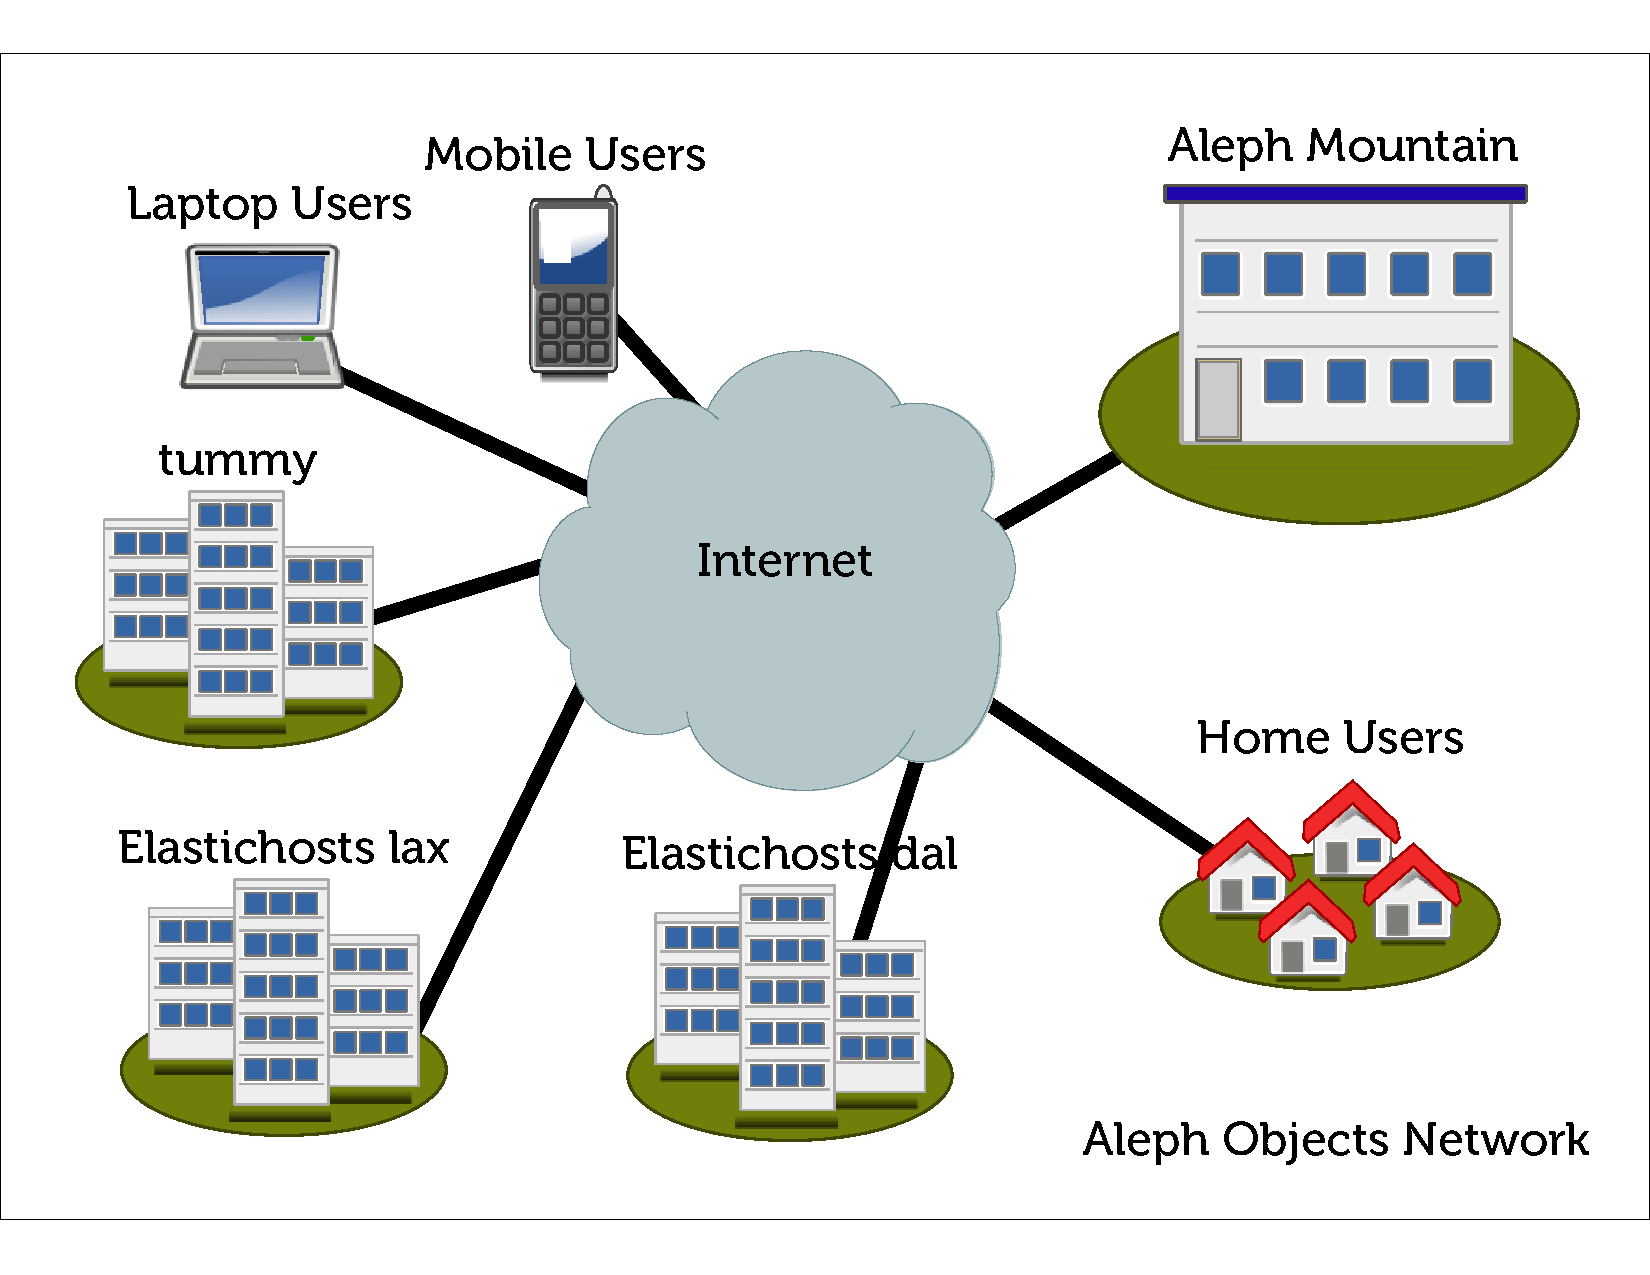
\includegraphics[keepaspectratio=true,height=1.10\textheight,width=1.00\textwidth,angle=0]{ao-network-overview.pdf}
 \caption{Aleph Objects Network Overview, May, 2015}
 \label{fig:ao_net_overview}
\end{figure}

